\documentclass[border=10pt]{standalone}

\usepackage{tikz}
\usepackage{tikzsymbols}
\usetikzlibrary{calc,patterns,shapes.geometric}

\def\centerarc[#1](#2)(#3:#4:#5){\draw[#1] ($(#2)+({#5*cos(#3)},{#5*sin(#3)})$) arc (#3:#4:#5);}

\begin{document}
	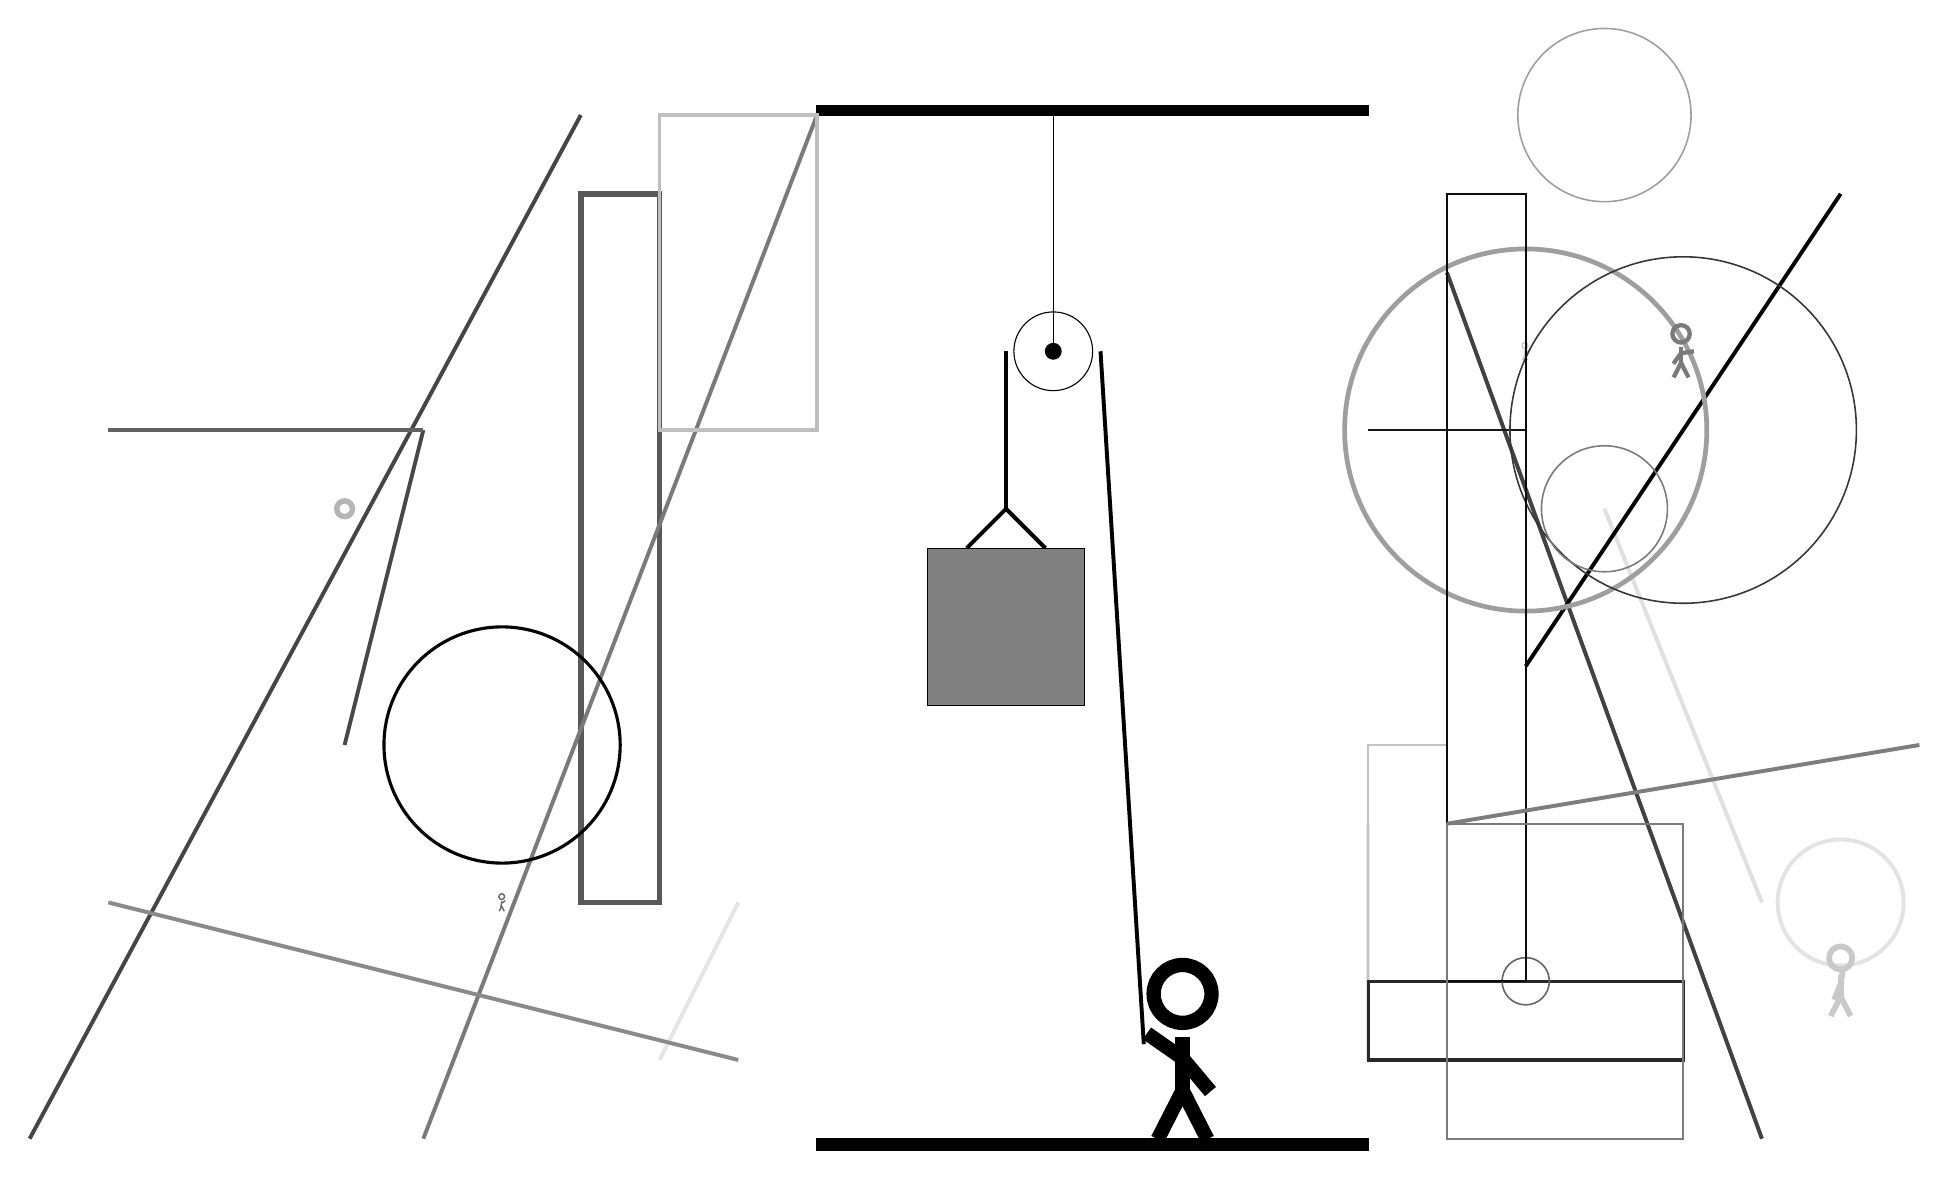
\begin{tikzpicture}
		%%%%% START %%%%%
		
		\draw[fill=black] (-2, 10) rectangle (5, 10.125);
		
		\draw (1, 7) circle (0.5);
		\draw[fill=black] (1, 7) circle (0.1);
		\draw (1, 10) -- (1, 7);
		
		\draw[line width=0.5mm] (-0.1, 4.5) -- (0.4, 5.0) -- (0.9, 4.5);
		\draw[fill=black!50] (-0.6, 4.5) rectangle (1.4, 2.5);
		
		\draw[line width=0.5mm] (0.4, 7) -- (0.4, 5.0);
		\centerarc[line width=0.5mm](1, 7)(0:180:0.6);
		\draw[line width=0.5mm](1.6, 7) -- (2.15, -1.8);
		
		\node at (2.6, -1.9) {\Strichmaxerl[10][-35][-50]};
		
		\node[line width=0.7mm, color=black!22] at (7, 7) {\Strichmaxerl[1][86][17]};
		
		\draw[line width=0.5mm, color=black!74](6, 8) -- (10, -3);
		\draw[line width=0.7mm, color=black!65] (-4, 0) rectangle (-5, 9);
		\draw[line width=0.5mm, color=black!73](-5, 10) -- (-12, -3);
		\draw[line width=0.5mm, color=black!52](-2, 10) -- (-7, -3);
		\draw[line width=0.5mm, color=black!12](8, 5) -- (10, 0);
		
		\draw[line width=0.3mm, color=black!91] (5, 6) rectangle (7, 6);
		\node[line width=0.3mm, color=black!59] at (-6, 0) {\Strichmaxerl[1][77][33]};
		\draw [line width=0.5mm, color=black!11](11, 0) circle (0.8);
		\draw [line width=0.2mm, color=black!38](8, 10) circle (1.1);
		\draw[line width=0.5mm, color=black!10](5, 1) -- (5, -2);
		
		\draw [line width=0.3mm, color=black!34](9, 8) circle (0.0);
		\draw[line width=0.5mm, color=black!99](7, 3) -- (11, 9);
		
		\draw[line width=0.4mm, color=black!25] (-2, 6) rectangle (-4, 10);
		\draw[line width=0.3mm, color=black!23] (5, -1) rectangle (6, 2);
		\draw [line width=0.6mm, color=black!38](7, 6) circle (2.3);
		
		\draw [line width=0.7mm, color=black!29](-8, 5) circle (0.1);
		
		\draw[line width=0.4mm, color=black!84] (5, -2) rectangle (9, -1);
		\draw[line width=0.5mm, color=black!72](-7, 6) -- (-8, 2);
		
		\draw [line width=0.2mm, color=black!79](9, 6) circle (2.2);
		\draw [line width=0.2mm, color=black!61](7, -1) circle (0.3);
		\draw[line width=0.5mm, color=black!10](-3, 0) -- (-4, -2);
		\node[line width=0.4mm, color=black!21] at (11, -1) {\Strichmaxerl[4][68][81]};
		\node[line width=0.5mm, color=black!52] at (9, 7) {\Strichmaxerl[3][54][8]};
		\draw [line width=0.2mm, color=black!52](8, 5) circle (0.8);
		
		\draw[line width=0.5mm, color=black!62](-7, 6) -- (-11, 6);
		\draw[line width=0.2mm, color=black!95] (6, 9) rectangle (7, -1);
		\draw[line width=0.5mm, color=black!51](6, 1) -- (12, 2);
		\draw [line width=0.4mm, color=black!99](-6, 2) circle (1.5);
		\draw[line width=0.5mm, color=black!46](-3, -2) -- (-11, 0);
		\draw[line width=0.3mm, color=black!52] (6, 1) rectangle (9, -3);
		
		
		\draw[fill=black] (-2, -3) rectangle (5, -3.15);
		
		%%%%% END %%%%%
	\end{tikzpicture}
\end{document}